\section{Determining the stability of operating performance points}
\label{sec:unstableOPPs}

In this section, we determine which OPPs are stable and which OPPs are unstable,
i.e. those in which the system operates normally and those which cause the system
to crash, respectively. Such a crash typically manifests as a kernel panic.
In particular, we would like to know which specific OPPs lie on the boundary
between the stable realm and the unstable realm. Henceforth, such an OPP is
referred to as a \textit{critical point}, and the voltage offset associated
with a critical point is called the \textit{critical voltage} of the frequency
associated with that same critical point. The following basic process lays out
how we can determine these critical points:

\begin{enumerate}
    \item \label{item:chooseFreq} Choose a frequency that has not yet been
        chosen from the set of possible frequencies, and set that as the current
        CPU frequency. If no previously unchosen frequency exists, we are done
        and have determined all the critical points.
    \item \label{item:computeSHA} Perform some fixed computational task, e.g.
        compute the SHA-1 hash of some predefined data. If the system crashes,
        record the current OPP as a critical point and go to step
        \ref{item:chooseFreq}.
    \item \label{item:undervolt} Decrease the CPU voltage by the smallest
        possible amount (i.e. $\frac{1}{1024}$~volts), then go to step
        \ref{item:computeSHA}.
\end{enumerate}

In practice, we expand upon this process in order to collect a more suitable
dataset. The process given above is repeated numerous times for each possible
frequency in order to obtain a reasonable sample size from which to determine
an average voltage offset which renders the system unstable for that frequency.
Ideally, this data collection would be automated, with the testbench running
through the process detailed above on boot, recording the tested OPPs to disk,
and rebooting after a system crash to repeat the process for different
frequencies as required. In practice, this is not possible, for the following
reasons:

\begin{itemize}
    \item any data that ought to be written to disk may not actually be flushed
        from memory to disk before the system encounters a kernel panic,
        resulting in loss of these data; and
    \item the system does not always reboot after encountering a kernel panic,
        contrary to the operating system's intended function of rebooting 30
        seconds after a kernel panic. In such situations, the machine must be
        reset manually.
\end{itemize}

Thus, to save time in collecting this data, we narrow down the range in which
the critical voltage lies for each frequency by only testing certain voltage
offsets. We then take the time to more precisely determine the critical voltage
for each frequency by testing all voltage offsets within this narrower range.
We do this with the aid of the \code{cpupower} and \code{undervolt} utilities
discuss in §\ref{sec:cpupower} and §\ref{sec:undervolt}, respectively.

The \code{undervolt} utility expects voltage offsets to be expressed in
millivolts (mV, units of $\frac{1}{1000}$~volts) rather than the MSR interface's
expected units of $\frac{1}{1024}$~volts. It then rounds the value given in
millivolts to the nearest multiple of $\frac{1}{1024}$~volts and writes the
appropriate value to the MSR. As such, the "smallest possible amount" mentioned
in step~\ref{item:undervolt} of the process above is taken as 1~mV rather than
$\frac{1}{1024}$~volts. The process we end up using is described by the
flowchart in Figure~\ref{fig:data-collection-flowchart}. Since we cannot fully
automate this process as discussed earlier, we collect the data by hand by
running through this process with the aid of a shell script,
\code{undervolt-test.sh}, the details of which are given in
§\ref{sec:undervolt-test.sh}.

\begin{figure}[!htb]
    \center{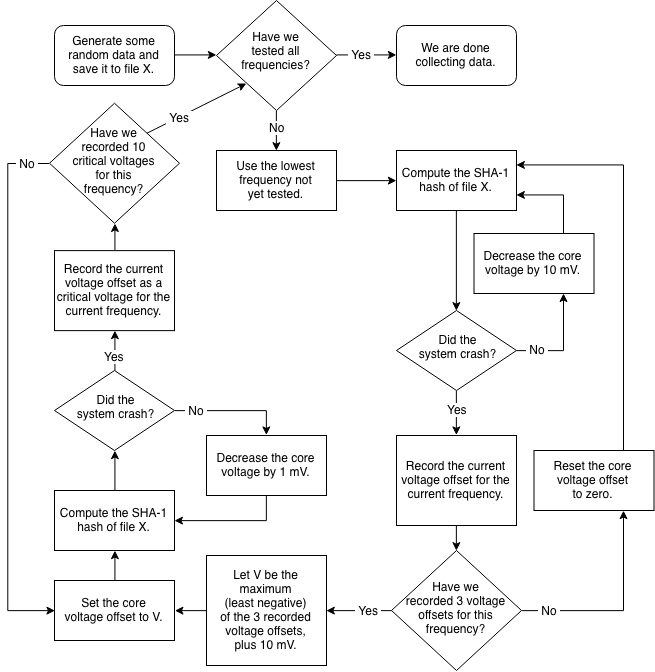
\includegraphics[width=\columnwidth,keepaspectratio]{data-collection-flowchart.png}}
    \caption{
        \label{fig:data-collection-flowchart}
        Flowchart describing how we collect data to determine the critical
        points.
    }
\end{figure}

In particular, for each frequency, we first find the critical voltage to the
nearest 10~mV, performing three (3) repetitions. We assume that the critical
voltage for the current frequency is bounded above by the maximum (least
negative) of these three samples plus 10~mV. We then find the critical voltage
to as much accuracy as is possible (i.e. to the nearest 1~mV) by testing every
possible voltage offset below this upper bound, performing ten (10) repetitions.
In Figure~\ref{fig:critical-points-graph}, we plot the mean, minimum, and
maximum of these 10 new data points for each possible frequency, which
collectively represent what the critical voltage is for that frequency.

\begin{figure}[!htb]
    \center{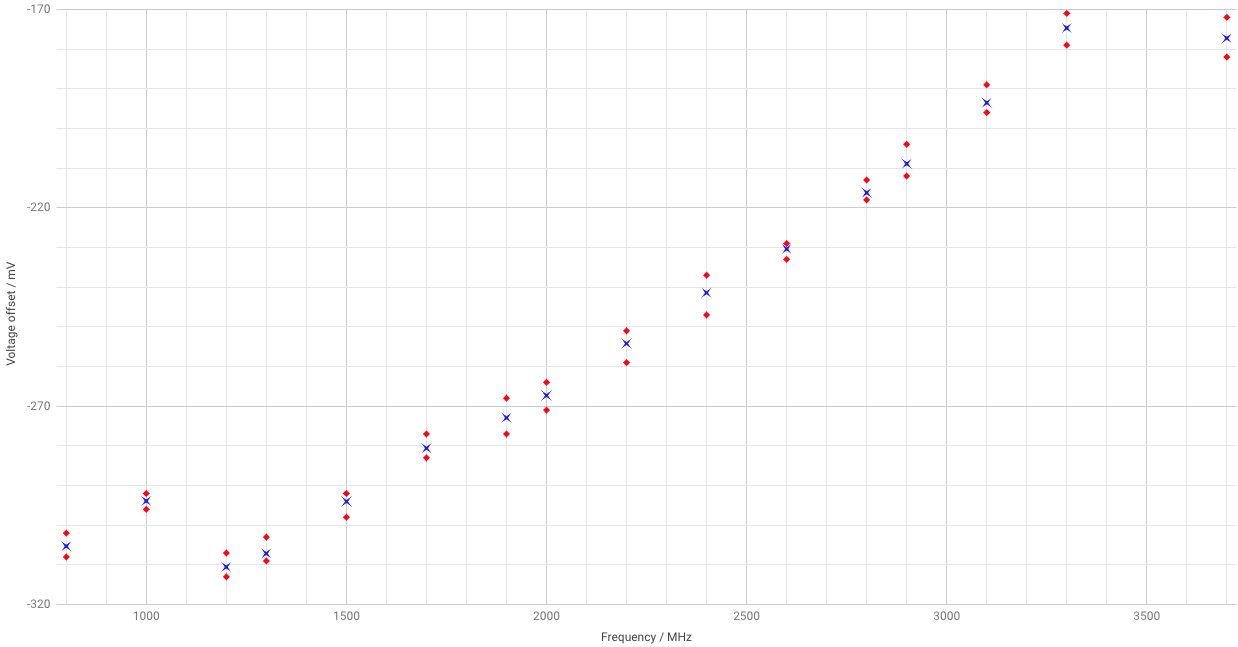
\includegraphics[width=\columnwidth,keepaspectratio]{critical-points-graph.png}}
    \caption{
        \label{fig:critical-points-graph}
        Graph plotting highest unstable voltage offset against frequency, using
        the data collected in determining the critical points. The blue cross
        for a given frequency is the mean of the voltage offsets recorded for
        that frequency. The red diamonds are the bounds for the corresponding
        error bars (maximum and minimum of the recorded voltage offsets).
    }
\end{figure}

Observe in Figure~\ref{fig:critical-points-graph} the clear trend between
frequency and the highest unstable voltage offset for a given frequency.
A trend line drawn for this dataset would separate the graph into two regions:

\begin{itemize}
    \item the upper-left region, which contains all the stable OPPs; and
    \item the lower-right region, which contains all the unstable OPPs.
\end{itemize}
